%Prelim, Chapter 1
% by Rachel Slaybaugh

\chapter{Introduction}
\label{sec:Chp1}

Nuclear technology plays an important role in society, particularly within the field of energy generation. More nuclear reactors are being constructed, existing designs are being refined, and new plants are being developed. For progress to continue in these areas, the modeling of nuclear systems must also progress. 

The neutron transport equation describes ``where all the neutrons are'' in a nuclear system. The more accurately this is known, the more accurately new systems can be developed. This means that solutions to the transport equation are needed in high-fidelity in all parts of phase space. Very large computers are now available to perform such high-fidelity calculations, but most existing solution methods are not able to take full advantage of new computer architectures and converge slowly for some kinds of problems.  

The goal of this research is to accelerate transport calculations with methods that use new computers fully and effectively, facilitating the design of better nuclear systems. Three complimentary methods have been implemented that accomplish this goal. In the chapters that follow this one, background information, past work, mathematics and implementation, and results will be discussed for each method in turn. 

This introductory chapter is intended to provide the foundation of this document. The types of neutron transport problems that have been, are, and could be solved are discussed first, including why such problems matter. This is followed by a presentation of the transport equation and its discretization. Finally, the way each method contributes to meeting the overall goal of this work is outlined. 

%--------------------------------------------------------------------------------
%--------------------------------------------------------------------------------
\section{Motivation}
The problems typically of interest in the nuclear engineering community are of large scale, with many independent variables representing the pertinent nuclear physics. Some of the most important applications are finding reactor core power distributions for cooling and safety needs, determining the criticality state of the reactor, and predicting isotope depletion. All of these applications require high-resolution neutron flux spectra, where flux is the number of particles per unit length squared per second in some portion of phase of space. Commercial light water reactors can have core heights of three to four meters and contain anywhere from 700 to 1200 fuel bundles \cite{Fennern2006}. Geometrically large shielding applications are commonly of interest as well. To obtain the needed quantities with sufficient precision and resolution, the size of required calculations can become quite large. 

Solving the full steady-state transport equation, which depends on location, energy, and solid angle, is computationally intensive. For a reasonable discretization of reactor-type calculations, $10^{8}$ coupled algebraic equations could easily be required. In the past, such large calculations were generally intractable because of computer hardware limitations: lack of memory and processing capability. There was simply not enough space to store all of the required data, and it would take too long to conduct the number of floating point operations (flops) needed. Calculations with fine enough discretizations to get high-resolution answers were impossible to perform using the transport equation \cite{Duderstadt1976}. 

Accordingly, simplifying approximations were used to solve problems in practice. Approximations include modeling reactor geometries in one or two dimensions rather than three; approximating neutron sources as isotropic; approximating neutron scattering as isotropic; eliminating the angular component of the solution through the diffusion approximation (discussed in Appendix \ref{sec:AppendixA}); physically truncating geometries by taking advantage of geometric symmetries or near symmetries, particularly for reactor cores with repeated lattice structures; and suppressing energy dependence or using very few energy groups \cite{Duderstadt1976}.

While all such approximations can be appropriate and give good results in some situations, they are generally not as accurate as solving the full, finely discretized transport equation. The way the nuclear industry has compensated for approximate answers is by building conservative margins into designs by using thicker shields, lower operating powers, larger safety margins, and so on. All of this costs money, which is of crucial import since economic competitiveness may be the largest barrier to the construction of new nuclear plants and, correspondingly, provision of emissions-free energy. Having higher-fidelity neutron fluxes could influence design bases and have a meaningful impact on current reactor operations and new reactor designs. 

%--------------------------------------------------------------------------------
\subsection{Problems of Interest}
To get more accurate fluxes, typical transport problems today are three-dimensional, have up to thousands $\times$ thousands $\times$ thousands of mesh points, use up to $\sim$150 energy groups, include accurate expansions of scattering terms, and are solved over many directions. Some examples of problems solved recently using discrete ordinates codes on parallel machines are shown next. The exact meaning of the expansions will become clear in the next section.
\begin{itemize}
  \item In 1998, 30 million unknowns\footnote{In each example the number of unknowns assumes one spatial unknown per cell; some spatial discretizations result in more than one spatial unknown per cell.}: a 3-D time dependent shielding problem where a 10 $\times$ 10 $\times$ 10 cm innermost region containing water and a uniform source is surrounded by 10 cm of iron, which is surrounded by 30 more cm of water. Three energy groups, a 50 $\times$ 50 $\times$ 50 Cartesian mesh, $S_{8}$ scattering quadrature, $P_{0}$ scattering expansion, and the adaptive weighted diamond difference method were used \cite{Alcouffe1998}.
  \item In 2004, 1.62 million unknowns: a cylinder with a 3.5 cm radius and 9 cm length containing layers of boron-10, water, and highly enriched uranium was solved with 13,500 cells, $S_{4}$ Chebyshev-Legendre quadrature, and five energy groups \cite{Warsa2004a}. 
  \item In 2010, 78.5 billion unknowns: a Pressurized Water Reactor (PWR)-900 with two groups, a 578 $\times$ 578 $\times$ 700 mesh, using $S_{16}$ level-symmetric quadrature, and with $P_{0}$ scattering was solved \cite{Davidson2010}. 
\end{itemize}
%
The size and scope of problems of interest have been increasing as larger computer resources have made it possible to solve them. 

The next phase of challenging problems are even more highly refined. High-fidelity, coupled, multi-physics calculations are the new ``grand challenge'' problems for reactor analysis. Of particular interest in nuclear systems is feedback between neutronics and thermal-hydraulics. A recent INCITE grant was awarded to spatially quantify data uncertainties in 3-D Boiling Water Reactor assembly calculations. When neutron transport is coupled to a fluid dynamics code it is important to know whether or not homogenizing the materials in the subchannels being analyzed will have a large impact. Such uncertainty studies will require spatial meshes exceeding 500 million elements \cite{Evans2009a}. Calculations of this detail present the next generation of challenges for computational neutronics. 

%--------------------------------------------------------------------------------
\subsection{Enabling Technology}
Nuclear transport computation began in the age of run tapes and punch cards with widely used codes being written in advanced programming languages such as FORTRAN IV \cite{Fortran1998}. Computer technology has evolved quickly and radically since that time. Now there are machines like Jaguar, which consists of two partitioned machines, the Cray XT4 and the Cray XT5. Jaguar has 84 XT4 cabinets containing 7,832 quad-core Opteron 1354 "Budapest" processors, each with eight gigabytes of DDR2-800 memory. The 200 XT5 cabinets have 37,376 six-core Opteron 2435 "Istanbul" processors with 16 gigabytes of memory per node. The machine has a total of 362 terabytes of high-speed memory \cite{Sciences2010}. A table of machine parameters can be seen in Figure~\ref{fig:jaguar}. 

\begin{figure}[!h]
  \begin{center}
    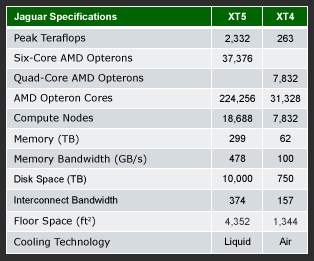
\includegraphics [width=0.55\textwidth, height=0.35\textheight ] {jaguarSpecs09}
  \end{center}
  \caption{Jaguar Machine Specifications \cite{Sciences2010}}
  \label{fig:jaguar}
\end{figure}

While the fastest computer in the world in 2010 may not be the best example of what is standard, machines on which parallel codes can be run are widely available and are becoming faster over time. Access to such machines has changed the landscape of the types of neutron transport problems that can be solved practically. 

Whenever an equation is being mathematically approximated, errors can be introduced that are inherent in the approximation. These errors are present regardless of machine roundoff, phase space discretization, etc. and cannot be changed without changing the approximation. Accepting this mathematical limit as a given, the factor that can be changed to improve calculations is machine architecture. This means that the quality of calculations for a given method is ultimately limited by computers. The research presented here is intended to provide methods that can take full advantage of these new computers, pushing back the frontier of limiting calculations.

%--------------------------------------------------------------------------------
%--------------------------------------------------------------------------------
\section{The Transport Equation}
To understand the methods that were developed for this work and how they will enable the use of leadership-class hardware, the mathematical details of the transport equation must be discussed first. This section does this for neutrons in steady-state systems. 

Neutrons can have many different kinds of interactions that influence a system's behavior. These interactions are described by cross sections, which reflect the likelihood of a particular interaction occurring and are given in units of inverse length. Of particular interest is the total cross section, $\Macro$, which includes all possible interactions; the scattering cross section, $\Macro_{s}$, where scattering can change the momentum and kinetic energy of a neutron; and the fission cross section, $\Macro_{f}$.   

Fission is the process through which a nucleus splits into (typically two) smaller atoms. Through this process a relatively large amount of energy is released along with several neutrons. These neutron are available to go on to cause other fissions, creating a chain reaction. The quantity $\nu$ is the average number of neutrons released per fission. Most of the energy released from fission is kinetic, which creates the heat used to make electricity \cite{Lewis1993}.  

If fission is occurring, it is often of interest to know the asymptotic behavior of the system. A reactor is called ``critical'' if the chain reaction is self-sustaining and time-independent. If the system is not in equilibrium then the asymptotic neutron distribution, or the fundamental mode, will grow or decay exponentially over time. A convenient way to capture this behavior is to assume $\nu$ can be adjusted to obtain a time-independent solution by replacing it with $\frac{\nu}{k}$, where $k$ is the parameter expressing the deviation from critical. 

This substitution changes the transport equation into an eigenvalue problem. A spectrum of eigenvalues can be found, but at long times only the non-negative solution corresponding to the largest real eigenvalue will dominate. The eigenproblem can be written as:
%
\begin{align}
   [\hat{\Omega} \cdot \nabla + \Macro(\vec{r}, E)] \psi(\vec{r}, \hat{\Omega}, E)  &=  \int dE' \int d\hat{\Omega'} \:\Macro_{s}(\vec{r}, E' \to E, \hat{\Omega'} \cdot \hat{\Omega}) \psi(\vec{r}, \hat{\Omega'}, E') \nonumber \\
&+\frac{ \chi(E)}{k} \int dE' \:\nu \Macro_{f}(\vec{r}, E') \int d\hat{\Omega'} \:\psi(\vec{r}, \hat{\Omega'}, E') \:,
\label{eq:neutron transport}
\end{align}
%
\noindent where the quantities are at location $\vec{r}$, traveling in directions $\hat{\Omega}$, and at energy E and are defined as:
\begin{list}{}{\hspace{2em}}
  \item $\psi(\vec{r}, \hat{\Omega}, E)$ is the angular neutron flux in neutrons per unit length squared per steradian and expresses where all the neutrons are in phase space, 
  \item $\chi(E)$ is the fission spectrum and specifies the energy distribution of neutrons born from fission,
  \item $k$ can be thought of as the asymptotic ratio of the number of neutrons in one generation to the number in the next \cite{Lewis1993}.
\end{list}

If fission is not present the transport equation becomes a fixed source rather than eigenvalue problem. The term containing $k$ is replaced by an external source, $q_{ex}(\vec{r}, \hat{\Omega}, E)$, and the equation becomes a standard linear system. 

A brief aside about some properties of the transport equation will aid in understanding the challenge of finding solution techniques that work in all cases. In a void, the transport equation is like a hyperbolic wave equation. For highly-scattering regions where $\Macro_{s}$ is close to $\Macro$, the equation becomes elliptic for the steady-state case. If the scattering is forward-peaked then the equation is parabolic. All of these classes of equations have different solution strategies. The equation is linear, though non-linearities can be introduced if temperature-dependence of cross sections and other similar physics are considered \cite{Adams2002}.  The non-linear considerations are beyond the scope of this work and only the linear case is considered here.

To numerically solve Equation \eqref{eq:neutron transport} it is discretized in space, angle, and energy. This work uses the multigroup approximation, the scattering term is expanded in Legendre polynomials, and discrete ordinates are used to treat direction of neutron travel. There are many spatial differencing methods available, the discussion of which are beyond the scope of this document as the proposed work is not dependent upon the spatial discretization employed. To ensure the new methods apply to the most general cases it will be assumed that the matrices resulting from discretization are not necessarily symmetric. 

%--------------------------------------------------------------------------------
\subsection{Multigroup Approximation}
The first variable to discretize is energy. In the multigroup approximation, the energy range of interest is broken into $G$ groups. The neutron flux is constant in energy over each group. The groups are ordered such that the highest energy group bound corresponds with $g = 0$, meaning group 1 is defined over $E_{1}$ to $E_{0}$, and the lowest energy bound corresponds with $g = G$. On this grid the group angular flux is defined as: 
%
\begin{equation}
  \psi_{g}(\vec{r},\hat{\Omega}) = \int_{g} dE \:\psi(\vec{r}, \hat{\Omega}, E) = \int_{E_{g}}^{E_{g-1}}dE \:\psi(\vec{r}, \hat{\Omega}, E) \:.
\end{equation}

Justification of this definition comes from assuming the angular flux within each energy group can be approximated by the product of the group flux and a known function: $\psi(\vec{r}, \hat{\Omega}, E) \approx f(E)  \psi_{g}(\vec{r},\hat{\Omega})$ for $E_{g} < E \le E_{g-1}$. The function is normalized for a specific group $g$ such that $\int_{g' = g} dE \:f(E) = 1$ and $\int_{g' \ne g} dE \:f(E) = 0$. The details of $f$ are isotope-dependent and can be garnered from nuclear data. With this notation, group quantities are defined as:

\indent $\Macro_{g}(\vec{r}) = \int_{g} dE \:\Macro(\vec{r}, E) f(E)$, \\
\indent $\nu \Macro_{fg}(\vec{r}) = \int_{g} dE \:\nu \Macro_{f}(\vec{r}, E) f(E)$, \\ 
\indent $\Macro_s^{gg'}(\vec{r}, \hat{\Omega'} \cdot \hat{\Omega}) = \int_{g} dE \:\int_{g'} dE' \:\Macro_{s}(\vec{r}, E' \to E, \hat{\Omega'} \cdot \hat{\Omega})  f(E')$ is the scattering from $g'$ into $g$, \\
\indent $\chi_{g} = \int_{g} dE \:\chi(E)$, and \\
\indent $q^{e}_{g}(\vec{r}, \vOmega) = \int_{g} dE \:q_{ex}(\vec{r}, \hat{\Omega}, E)$.

\noindent Using these terms, the eigenvalue form of Equation \eqref{eq:neutron transport} can be rewritten for each group $g$ as seen in \eqref{eq:group-transport} \cite{Lewis1993}. Using more energy groups represents the physics in the cross sections more accurately, but also increases the cost of a calculation in terms of both operations and storage. 
% 
\begin{align}
   [\hat{\Omega} \cdot \nabla + \Macro_{g}(\vec{r})] \psi_{g}(\vec{r}, \hat{\Omega})  &=  \sum_{g'=1}^{G} \int d\hat{\Omega'} \:\Macro_s^{gg'}(\vec{r}, \hat{\Omega'} \cdot \hat{\Omega}) \psi_{g'}(\vec{r}, \hat{\Omega'})  \nonumber \\
&+ \frac{\chi_{g}}{k}   \sum_{g'=1}^{G} \nu \Macro_{fg'}(\vec{r}) \int d\hat{\Omega'} \:\psi_{g'}(\vec{r}, \hat{\Omega'}) 
\label{eq:group-transport}
\end{align}

%--------------------------------------------------------------------------------
\subsection{Scattering Discretization}
In Equation \eqref{eq:group-transport} the scattering cross section is a complicated function of angle. Simplifying this term will make the system easier to solve. Because of rotational symmetry of nuclear collisions, $\Macro_{s}$ is only a function of the cosine between the incoming and outgoing angles. This allows the scattering cross section to be written as a series expansion of Legendre polynomials as follows, where the the spatial variable has been supressed:
%
\begin{equation}
  \sigg{}(\vOmega' \cdot \vOmega) = \sum_{l=0}^{N} \frac{2l+1}{4\pi} P_{l}(\vOmega' \cdot \vOmega)\sigg{l} \:.
\end{equation}

The addition theorem of spherical harmonics can be used to evaluate the Legendre function, $P_{l}(\vOmega' \cdot \vOmega)$, with spherical harmonic terms, $Y_{lm}$. These can then be expanded into real and imaginary components. The imaginary components must be zero since scattering must be real. All of this gives:
%
\begin{equation}
  P_l(\vOmega' \cdot \vOmega) = \frac{4\pi}{2l+1} \Bigl[ Y^e_{l0}(\vOmega) Y^e_{l0}(\vOmega') + \sum_{m=1}^l \bigl( Y^e_{lm}(\vOmega) Y^e_{lm}(\vOmega') + Y^o_{lm}(\vOmega) Y^o_{lm}(\vOmega') \bigr) \Bigr]\:.
\end{equation}
%
The $Y^e$ and $Y^o$ terms obey the following orthogonality relationships: $\int d\vOmega \:Y^{e}_{lm}(\vOmega)Y^{e}_{l'm'}(\vOmega) = \frac{1}{2}(1 + \delta_{m0})\delta_{ll'}\delta_{mm'}$ and $\int d\vOmega \:Y^{o}_{lm}(\vOmega)Y^{o}_{l'm'}(\vOmega) = \frac{1}{2}(1 - \delta_{m0})\delta_{ll'}\delta_{mm'}$. The spherical harmonics therefore form an orthonormal basis in which the Legendre polynomials are expressed \cite{Evans2009}, \cite{Lewis1993}. 

By putting all of this information together, the scattering source can be expressed as: 
%
\begin{equation}
  q^g_{s} (\vec{r}, \vOmega) = \sum_{g'=1}^G \sum_{l=0}^N \sigg{l}(\vec{r}) \Bigl[ Y^e_{l0}(\vOmega) \evenp_{l0}(\vec{r}) + \sum_{m=1}^l \bigl( Y^e_{lm}(\vOmega) \evenp_{lm}(\vec{r}) + Y^o_{lm}(\vOmega) \oddp_{lm}(\vec{r}) \bigr) \Bigr]\:.
   \label{eq:mg-scattering-source}
\end{equation}
%
In Equation \eqref{eq:mg-scattering-source} two terms, called the even and odd flux moments, have been used:
%
\begin{alignat}{3}
  \even_{lm} &= \int_{4\pi} d\vOmega' \:Y^e_{lm}(\vOmega') \psi^g(\vOmega') \:, \quad& m\ge 0\:,\qquad \text{even} \:, \label{eq:even-flux}\\
  %
  \odd_{lm} &= \int_{4\pi} d\vOmega' \:Y^o_{lm}(\vOmega')\psi^g(\vOmega') \:, \quad& m>0 \:,  \qquad \text{odd} \label{eq:odd-flux} \:.
\end{alignat}
%
The external source can be similarly discretized if desired, making the two sources consistent with one another. The full details of these expansions and bases can be found in \cite{Evans2009}. 

The multigroup, anisotropic scattering source found in Equation \eqref{eq:mg-scattering-source} is characterized by the order of Legendre scattering, $P_{N}$. For a given Legendre expansion there are $(N + 1)^{2}$ flux moments. Using more moments represents scattering more accurately, but increases the cost of calculation \cite{Evans2009}.  

%--------------------------------------------------------------------------------
\subsection{Discrete Ordinates Approximation}
The next area of phase space to discretize is direction. The discrete ordinates or \Sn approximation is a collocation method that is used to express the transport equation on a discrete set of $n$ ordinates, where the ordinates are described by angles and represent direction of neutron travel. A collocation method represents a continuous function on a finite set of collocation points using a linear combination of basis functions. The approximate solution must satisfy the differential equation at those collocation points \cite{Heath2002}. 

For the transport equation, the basis functions are the angular fluxes along specific directions and the collocation points are the angle sets. The linear combination is done by weighting the basis functions using a quadrature set. 

To implement this, the transport equation is written for neutrons traveling in $d\vOmega$ about direction $\vOmega_{a}$. Now $\psi^{g}_{a}$ can be defined as $\psi^{g}(\vOmega_{a})$, and the angular flux can be related to the scalar flux as $\phi^{g} = \sum_{a=1}^{n}\psi^{g}_{a}w_{a}$. Using these terms, including the discretized scattering source and suppressing spatial dependence, Equation \eqref{eq:group-transport} becomes:
%
\begin{align}
 \bigl( \vOmega_{a} \cdot \nabla + \Macro_{g} \bigr) \psig_{a} = \sum_{g' = 1}^{G} \sum_{l=0}^{N} \sigg{l} \bigl[ Y^{e}_{l0}(\vOmega_{a}) \evenp_{l0} &+ \sum_{m=1}^{l} \bigl( Y^{e}_{lm}(\vOmega_{a}) \evenp_{lm} + Y^{o}_{lm}(\vOmega_{a}) \oddp_{lm} \bigr) \bigr] \nonumber \\
 &+ \frac{\chi^{g}}{k} \sum_{g'=1}^{G} \nu \Macro_{f}^{g'}\phi^{g'} \:,
  \label{eq:mg-sn-transport}
\end{align}

The quadrature weights, $w_{a}$, are defined such that $\int_{4 \pi} d\vOmega =  \sum_{a=1}^{n}w_{a} = 4 \pi$. One of the choices in the \Sn approximation is what quadrature set to use. The number of unknowns contributed by discretization of direction is determined by the quadrature set. For example, level-symmetric quadrature gives $n = N(N+2)$ unknowns for an \Sn approximation. The scalar flux is also collocated on the ordinates using the desired quadrature set to linearly combine the angular flux basis functions \cite{Evans2009}. This results in the flux moments:
%
\begin{align}
  \even_{lm} &= \sum_{a=1}^{n}Y^e_{lm}(\vOmega'_a)\psi^g_a w_a\:,
  \label{eq:even-flux-quad-int}\\
  \odd_{lm} &= \sum_{a=1}^{n}Y^o_{lm}(\vOmega'_a)\psi^g_a w_a\:.
  \label{eq:odd-flux-quad-int}
\end{align}

%--------------------------------------------------------------------------------
\subsection{Operator Form}
Now that the transport equation has been discretized, it can be expressed in operator notation. Using the operator form of the transport equation will facilitate the presentation of the solution techniques discussed in the remainder of this document. In general, uppercase bolded letters will indicate matrices and lowercase italicized letters will indicate vectors and scalars. The following operators are used to express the transport equation:\\
%
\indent $\mathbf{L} = \vOmega \cdot \nabla + \Macro$ is the transport operator, \\
\indent $\mathbf{M}$ is the operator that converts harmonic moments into discrete angles, \\
\indent $\mathbf{S}$ is the scattering matrix, \\
\indent $f$ contains the fission source, $\nu \Macro_{f}$; $\mathbf{F} =\mathbf{\chi} f^{T}$, \\ 
\indent $\mathbf{D} = \ve{M^{T}}\ve{W} = \sum_{a=1}^{n}Y^{e/o}_{lm}w_{a}$ is the discrete-to-moment operator. 

With this notation Equation \eqref{eq:mg-sn-transport} can be written as \eqref{eq:operator-form}; it can be formulated as a fixed source problem by replacing the fission term with $\ve{M}q_{e}$. This has two unknowns, the angular flux and the moments, which are related by the discrete-to-moment operator as seen in Equation \eqref{eq:moments}.
%
\begin{align}
  \mathbf{L} \psi &= \mathbf{MS}\phi + \frac{1}{k}\mathbf{MF}\phi \label{eq:operator-form}\\
  \phi &= \mathbf{D}\psi 
  \label{eq:moments}
\end{align}
The typical strategy for solving Equation \eqref{eq:operator-form} is to combine it with \eqref{eq:moments} and form one equation involving only the moments, where $Q$ is comprised of the fixed or fission source: 
\begin{equation}
   (\ve{I} - \ve{DL}^{-1}\ve{MS})\phi = Q \:.
\end{equation}  
This is solved for $\phi$ from which $\psi$ can be determined at the end of the calculation.

The size of the operators can be defined in terms of the granularity of discretization: \\
%
\indent $G$ = number of energy groups, \\
\indent $t$ = number of moments, \\
\indent $n$ = number of angular unknowns, \\
\indent $c$ = number of cells, \\
\indent $u$ = number of unknowns per cell, which is determined by spatial discretization. \\
%
These can be combined to define $a = G \times n \times c \times u$ and $f = G \times t \times c \times u$. Using $a$ and $f$, Equation \eqref{eq:operator-form} can be presented in terms of operator size: $(a \times a)(a \times 1) = (a \times f) (f \times f) (f \times 1) + (a \times f) (f \times f) (f \times 1)$. The index variables, their meaning, and their ranges are shown in Table \ref{table:index}. 
%
\begin{table}[!h]
\caption{Meaning and Range of Indices Used in Transport Discretization}
\begin{center}
\begin{tabular}{l c c c c}
\hline
Variable & Symbol & First & Last \\[0.5ex]
\hline
Energy & g & 1 & G \\
Solid Angle & a & 1 & n \\
Space & suppressed & n/a & n/a \\
Legendre moment ($P_{N}$) & $l$ & 0 & N \\
Spherical harmonic moment ($Y$) & m & 0 & $l$ \\
\hline
\end{tabular}
\end{center}
\label{table:index}
\end{table}
%

The structures of the vectors and matrices are shown in the next few equations as this will make some of the proposed methods easier to understand and visualize \cite{Evans2009}. The angular flux vector is explicitly written first, where for each discrete angle, $a$, and energy group, $g$, the set of angular fluxes, $ \psi^g_a$, includes all spatial unknowns.
%
 \begin{align}
    \psi &=     \begin{pmatrix}
    [\psi]_{1} & [\psi]_2 & \cdots & [\psi]_g & \cdots [\psi]_{G} 
  \end{pmatrix}^T  \:, \qquad \text{and} \nonumber \\
  %
    [\psi]_g &= \begin{pmatrix}
    \psi^g_1 & \psi^g_2& \cdots & \psi^g_a & \cdots \psi^g_n 
  \end{pmatrix}^T \:.  \nonumber 
\end{align}
%
\begin{alignat}{2}
  \mathbf{M} &=    \begin{pmatrix}
      [\ve{M}]_{11} & 0 & 0 & \cdots & 0 \\
      0 & [\ve{M}]_{22} & 0 & \cdots & 0 \\
      0 & 0 & [\ve{M}]_{33} & \cdots & 0 \\
      \vdots & \vdots & \vdots & \ddots   & \vdots \\
      0 & 0 & 0 & \cdots & [\ve{M}]_{GG} \\
    \end{pmatrix} \nonumber  \:,& \qquad
    %
  \mathbf{S}  =     \begin{pmatrix}
      [\ve{S}]_{11} & [\ve{S}]_{12} & [\ve{S}]_{13} & \cdots &
      [\ve{S}]_{1G} \\
      [\ve{S}]_{21} & [\ve{S}]_{22} & [\ve{S}]_{23} & \cdots &
      [\ve{S}]_{2G} \\
      [\ve{S}]_{31} & [\ve{S}]_{32} & [\ve{S}]_{33} & \cdots &
      [\ve{S}]_{3G} \\
      \vdots & \vdots & \vdots & \ddots & \vdots \\
      [\ve{S}]_{G1} & [\ve{S}]_{G2} & [\ve{S}]_{G3} & \cdots &
      [\ve{S}]_{GG}
    \end{pmatrix} \nonumber  \:,
 \end{alignat}
 %
 \begin{alignat}{2}
      \mathbf{F}  &=     \begin{pmatrix}
     \chi^{1}[\nu\Macro_{f}]^{1} &\chi^{1}[\nu\Macro_{f}]^{2} & \cdots &
      \chi^{1}[\nu\Macro_{f}]^{G} \\
      \chi^{2}[\nu\Macro_{f}]^{1} &\chi^{2}[\nu\Macro_{f}]^{2} & \cdots &
      \chi^{2}[\nu\Macro_{f}]^{G}\\
      \vdots & \vdots & \ddots & \vdots \\
      \chi^{G}[\nu\Macro_{f}]^{1} &\chi^{G}[\nu\Macro_{f}]^{2} & \cdots &
      \chi^{G}[\nu\Macro_{f}]^{G}\\
    \end{pmatrix} \:, \nonumber & \qquad
    %
  [\ve{S}]_{gg'} = \begin{pmatrix}
    \sigg{0} & 0 & \cdots & 0  \\
    0 & \sigg{1} & \cdots & 0 \\
    \vdots & 0 & \ddots  & \vdots \\
     0 & 0 & \cdots & \sigg{N}
  \end{pmatrix}\:, \nonumber
 \end{alignat}
    %
\begin{equation}    
   [\ve{M}]_{gg} = \begin{pmatrix}
    \Ye{00}{1} & \Ye{10}{1} & \Yo{11}{1} & \Ye{11}{1} & 
    \Ye{20}{1} & \cdots & \Yo{NN}{1} & \Ye{NN}{1} \\
    \Ye{00}{2} & \Ye{10}{2} & \Yo{11}{2} & \Ye{11}{2} & 
    \Ye{20}{2} & \cdots & \Yo{NN}{2} & \Ye{NN}{2} \\
    \Ye{00}{3} & \Ye{10}{3} & \Yo{11}{3} & \Ye{11}{3} & 
    \Ye{20}{3} & \cdots & \Yo{NN}{3} & \Ye{NN}{3} \\
    \vdots     & \vdots     & \vdots     & \vdots     & 
    \vdots     &  \ddots    & \vdots     & \vdots     \\
    \Ye{00}{n} & \Ye{10}{n} & \Yo{11}{n} & \Ye{11}{n} & 
    \Ye{20}{n} & \cdots & \Yo{NN}{n} & \Ye{NN}{n}
  \end{pmatrix}\:. \nonumber \\
\end{equation}

\noindent Note that $[\ve{M}]_{11} = [\ve{M}]_{22} =  \hdots = [\ve{M}]_{GG} = [\ve{M}]$. These are written with subscripts to simplify the visualization of which blocks correspond to which equations and multiply which other blocks. 

%--------------------------------------------------------------------------------
\subsection{Solution Procedure}
Once the matrices are multiplied together, a series of single-group equations that are each only a function of space and angle result:
%
\begin{equation}
  \begin{aligned}
    \ve{L}[\psi]_1 &= [\ve{M}]\bigl([\ve{S}]_{11}[\phi]_1 + 
    [\ve{S}]_{12}[\phi]_2 + \ldots + [\ve{S}]_{1G}[\phi]_G\bigr) + 
    \frac{1}{k}[\ve{M}]\sum_{i=1}^{G}[\ve{F}]_{1i}[\phi]_{i} \:, \\
    %%
    \ve{L}[\psi]_2 &= [\ve{M}]\bigl([\ve{S}]_{21}[\phi]_1 + 
    [\ve{S}]_{22}[\phi]_2 + \ldots + [\ve{S}]_{2G}[\phi]_G\bigr) + 
     \frac{1}{k}[\ve{M}]\sum_{i=1}^{G}[\ve{F}]_{2i}[\phi]_{i} \:, \\
    %%
    &\vdots\\
    %%
    \ve{L}[\psi]_G &= [\ve{M}]\bigl([\ve{S}]_{G1}[\phi]_1 + 
    [\ve{S}]_{G2}[\phi]_2 + \ldots + [\ve{S}]_{GG}[\phi]_G\bigr) + 
     \frac{1}{k}[\ve{M}]\sum_{i=1}^{G}[\ve{F}]_{Gi}[\phi]_{i} \:.
  \end{aligned}
  \label{eq:group-equations}
\end{equation}
%
Each ``within-group'' equation is solved for that group's flux. If the groups are coupled together, as they often are, then multiple ``multigroup'' solves over the coupled portion of the energy range may be required. If the eigenvalue is desired an additional ``eigenvalue'' solve is needed as well \cite{Evans2009}. The details of these steps will be discussed later as they relate to the new methods.  


%--------------------------------------------------------------------------------
%--------------------------------------------------------------------------------
\section{Meeting the Goal}
The fully discretized steady-state transport equation can become very large when trying to solve ``grand challenge'' types of problems. The continued improvement of computational resources has enabled the invention of massively parallel codes designed to work on leadership-class computers. The goal of this work is to develop and implement methods that will accelerate transport calculations by efficiently taking advantage of cutting-edge computer architectures. 

The code being used in this work is Denovo \cite{Evans2009}, a massively parallel discrete ordinates code being developed at Oak Ridge National Laboratory (ORNL). The code allows multiple combinations of spatial discretizations, quadrature sets, and solution methodologies. Denovo is three-dimensional; uses a non-uniform, structured, Cartesian grid; has a flexible front end; and is capable of writing and reading input parameters rapidly for high performance computing. 

At the outset of this work, Denovo could be decomposed for parallel computation in five of the six dimensions of phase space over which the steady-state transport equation is solved. The nature of the decomposition dictated how many cores Denovo could use efficiently. Studies presented in Chapter \ref{sec:Chp2} illustrate that this number of cores was not sufficient to solve real problems of interest. 

The original suite of solvers in Denovo included Source Iteration (SI) and Krylov methods as within group solvers, Gauss Seidel (GS) as a multigroup solver, and power iteration (PI) as an eigenvalue solver. These solvers have some significant limitations in many cases. Each method and its associated challenges will be described in detail in following chapters. 

Acceleration of Denovo has been accomplished by implementing three complimentary solution strategies. The first is a multigroup solver that allows Denovo to be decomposed in energy for fixed source problems such that multigroup solves can be parallelized in the energy dimension. This addition lets Denovo to take advantage of many more cores without significantly degrading the scaling. The \emph{multigroup Krylov solver} also converges more quickly than Gauss Seidel. This work is discussed in Chapter~\ref{sec:Chp2}.

The second strategy was to add an eigenvalue method with properties that can be superior to power iteration, particularly for loosely coupled problems. \emph{Rayleigh Quotient Iteration} (RQI) applies a shift to the equations that improves the eigenvalue convergence properties. The shift also increases the degree of effective group-to-group coupling. The multigroup Krylov solver enables RQI because it solves coupled groups efficiently and decomposes those coupled groups for energy parallelization. The details of this work are discussed in Chapter~\ref{sec:Chp3}.

The third step was to add a new physics-based preconditioner that is a multigrid method in energy. This capitalizes on the energy decomposition added by the first method. Since energy groups can be treated independently, they can be combined and re-separated in a multigrid fashion very easily. The preconditioner is applicable to both fixed source problems and eigenvalue calculations, and it reduces the number of iterations required for convergence. The \emph{multigrid in energy preconditioner} is discussed in Chapter~\ref{sec:Chp4}.

Fast and scalable codes are necessary for solving truly large and challenging neutron transport problems. This work developed methods that accelerate an existing transport code by allowing it to scale to hundreds of thousands of cores and converge in fewer iterations than its previous methods, thus enabling the development of new and useful nuclear energy systems. These methods may also be beneficial for the larger computational community.

\separatorpage{}  
